\chapter{Asking Wall Street Millionaires How To Make \$1 Million}

This chapter is built from a street interview rather than a blackboard lecture, but it still has a clear internal mathematics. The same probe is applied again and again: when did you make your first million, by what mechanism did it happen, and what would you tell somebody trying to do the same now? Out of that repeated questioning there emerges, not a single formula for wealth, but a sequence of operating models: persistence under refusal, centralization and scale in a service business, the distinction between a windfall and a durable flow, the economics of professional practice, the leverage of distribution, and finally the private-equity insistence on actual cash generation rather than decorative earnings. No validated technical screenshots survive for this episode, so the figures below are cautious transcript-based reconstructions.

\section{Opening Question, Search Friction, and the Cost of Access}

The lecture opens by promising answers before it gives us a method. We hear of finance, private equity, a television network in airports and hotels, and a year in which \$250 million was made. We also hear a smaller but equally important confession: somebody made a first million only about a decade ago, sold everything, and started over. The teaser therefore does not yet teach us how wealth works; it tells us that the sample will be varied.

Once the host stands on Wall Street and states the day's plan, the real structure becomes visible. We are going to ask the same question over and over and let the answers separate themselves. What stays fixed is the probe: age at the first million, line of business, and the advice one would now give to somebody trying to make a million dollars in the present world. What changes is access. Some people refuse, some evade, some answer with a joke, and some offer only a fragment before moving on.

That first stretch of the lecture matters more than it seems. It shows us that information is not simply sitting on the pavement waiting to be collected. It is carried by moving people, protected by schedules, and often released only under repeated contact. One passerby says only that he lives the dream; another refuses to stop; another dismisses the conversation entirely. Even these weak replies have a function. They teach us that before we get any mechanism of wealth, we must pay a search cost.

\section{From ``No'' to ``Not Yet''}

After the failed first day, the host pauses the hunt and interprets the failure. This is the lecture's first true update. The key point is not that refusal is pleasant; it is that refusal is not allowed to terminate the process. In the lecture's own idiom, ``no'' becomes ``not yet.'' Schematically, we may write
\begin{equation}
\text{No}_t \longmapsto \text{Not Yet}_{t+1}.
\end{equation}
This is a psychological rule, but also a procedural one.

\begin{figure}[h]
\centering
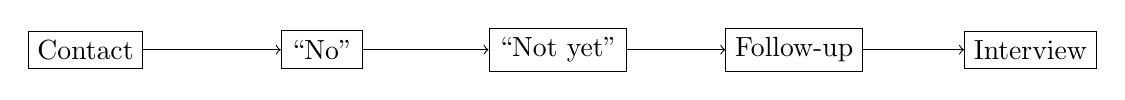
\begin{tikzpicture}
\node[draw, rectangle] (c) at (0,0) {Contact};
\node[draw, rectangle] (n) at (3,0) {``No''};
\node[draw, rectangle] (ny) at (6,0) {``Not yet''};
\node[draw, rectangle] (f) at (9,0) {Follow-up};
\node[draw, rectangle] (i) at (12,0) {Interview};
\draw[->] (c) -- (n);
\draw[->] (n) -- (ny);
\draw[->] (ny) -- (f);
\draw[->] (f) -- (i);
\end{tikzpicture}
\end{figure}

The point is exact. If the search process halts at the first rejection, then nothing deeper will ever be learned. If refusal is recoded as a delay state, the process stays alive long enough for a real case to appear. This is why the lecture's day-two reset is not merely motivational filler. It is the condition under which later mechanisms become observable.

We should also notice that this rule returns later in a different language. When the Reach TV founder is asked how to turn a likely no into a yes, he gives essentially the same answer: no is never no; it is always not yet. Thus the lecture introduces persistence first as field method and later recovers it as a sales principle. The same operator acts in both places.

\section{Dry Cleaning as a Scalable System}

The first substantial case is not a glamorous startup or a giant fund. It is dry cleaning. This is exactly the right place for the lecture to become concrete, because the mechanism is easy to state and hard to forget. The guest once had ten dry cleaners. When the host asks how one scales from one location to ten, the answer is immediate: own the factory.

\subsection{Question \& Answer}

\paragraph{Question.} How do we scale a small service business without building ten copies of the expensive core?

\paragraph{Answer.} We separate the edge of the business from the center. The storefront is not the true production site. It is a collection point, a tagging-and-bagging point, a retail interface. The factory is where the real processing is done. Once this separation is made, scale ceases to mean ``duplicate the whole business'' and begins to mean ``build one production core and many intake nodes.''

\begin{figure}[h]
\centering
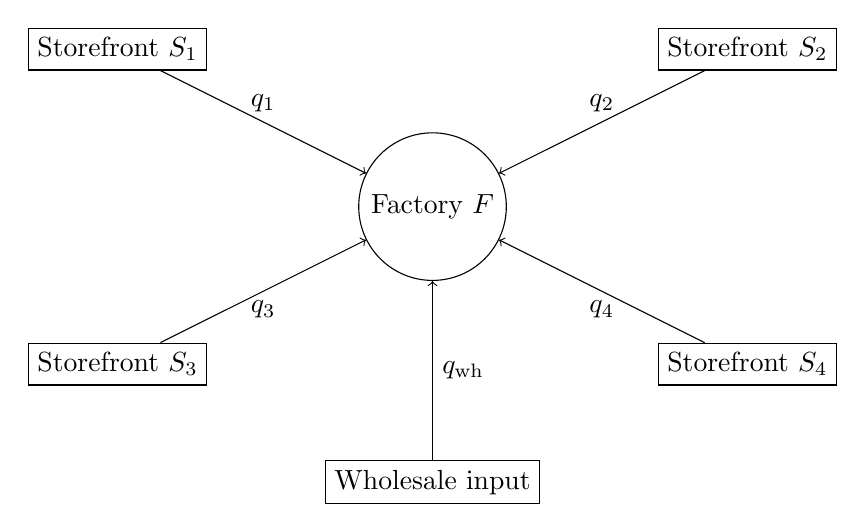
\begin{tikzpicture}
\node[draw, circle] (f) at (0,0) {Factory $F$};
\node[draw, rectangle] (s1) at (-4,2) {Storefront $S_1$};
\node[draw, rectangle] (s2) at (4,2) {Storefront $S_2$};
\node[draw, rectangle] (s3) at (-4,-2) {Storefront $S_3$};
\node[draw, rectangle] (s4) at (4,-2) {Storefront $S_4$};
\node[draw, rectangle] (w) at (0,-3.5) {Wholesale input};
\draw[->] (s1) -- node[above] {$q_1$} (f);
\draw[->] (s2) -- node[above] {$q_2$} (f);
\draw[->] (s3) -- node[below] {$q_3$} (f);
\draw[->] (s4) -- node[below] {$q_4$} (f);
\draw[->] (w) -- node[right] {$q_{\mathrm{wh}}$} (f);
\end{tikzpicture}
\end{figure}

The lecture does not write equations on a board, but the operating model is clean enough to formalize. Let $F$ denote the central factory, let $S_i$ denote storefront $i$, and let $q_i$ be the monthly intake at that storefront. Then the network throughput is
\begin{align}
Q &= \sum_{i=1}^{n} q_i, \qquad n_{\text{cleaners}} = 10, \\
R_{\text{network}} &= p_{\text{shirt}}\,Q, \qquad p_{\text{shirt}} \approx 1.99\ \text{USD}, \\
\Pi_{\text{network}} &= p_{\text{shirt}}Q - c_{\text{unit}}Q - C_F - \sum_{i=1}^{n} C_{S_i} - C_{\text{transport}}.
\end{align}
Here $C_F$ is the cost of the factory, $C_{S_i}$ is the local cost of storefront $i$, and $c_{\text{unit}}$ is the approximate processing cost per shirt-equivalent item. The transcript gives a rough unit-cost point of about \$0.40, though the exact wording at that moment is garbled.

\begin{remark}
This is an illustrative reconstruction, not a recovered profit-and-loss statement. The lecture supplies price, a rough marginal cost, a square-footage claim, and a monthly-profit claim, but it does not supply a full rent, labor, transportation, or utilization schedule.
\end{remark}

Still, the guest's numbers are strong enough to support a useful consistency check. He says one can operate a $500$ square foot site and still make roughly \$50{,}000 per month. If we momentarily suppress fixed costs and compute only the contribution margin, then
\begin{align}
m &= p_{\text{shirt}} - c_{\text{unit}} \approx 1.99 - 0.40 = 1.59\ \text{USD}, \\
Q^\star &\approx \frac{50{,}000}{1.59} \approx 3.14\times 10^4\ \text{garments/month}, \\
\frac{Q^\star}{30} &\approx 1.05\times 10^3\ \text{garments/day}.
\end{align}
This is not a proof that the location really nets exactly \$50{,}000 per month. It is better read as a scale check. The guest is telling us that the model presumes substantial throughput, and that throughput becomes believable precisely because the heavy production step is centralized.

The lecture then sharpens the point. Once the factory is sufficiently good, apparent competitors can become customers, because they too want wholesale processing. The structure therefore widens from a retail chain to a hub that can absorb outside volume. The deeper lesson is not about dry cleaning in particular. It is about architecture. One scales by controlling the indispensable center and lightening the edge.

Finally, the guest says he later moved from dry cleaning into tech because, in his words, there is no money like tech. The lecture is careful here. It does not retract the dry-cleaning model. It simply says that once one has learned how systems scale, the same taste for leverage will naturally look for larger arenas.

\section{From First Million to Durable Flow}

At this point the lecture refuses to stop at the making of money. The speaker asks the more difficult question: what keeps the flow going? The same guest, having explained how the first business scaled, is now asked what lesson he would give to someone trying to make a million dollars today. Before he answers the question of preservation directly, he inserts a prior discipline: be more interested than interesting. If one goes into a room merely trying to be the star, one learns less. That advice prepares the later shift from reaction to patience.

The next line is one of the lecture's hinges. We live, the guest says, in a world where people want a reaction right now. But sustainable wealth does not arrive in that way. A quick gain and a recurring flow are not the same object. If we write a stripped-down wealth identity,
\begin{equation}
W_{t+1} = W_t + CF_t - C_t,
\end{equation}
then the lecture's claim is that preservation is not secured merely by a single large $CF_t$. Preservation requires that the cash-generating mechanism endure, and that spending not accelerate merely because income once spiked. In particular,
\begin{equation}
\Delta W_t > 0 \qquad \Longleftrightarrow \qquad CF_t > C_t
\end{equation}
is a necessary condition for persistence, but the lecture wants us to notice that the most dangerous variable is often behavioral rather than technical.

\subsection{Question \& Answer}

\paragraph{Question.} If somebody makes a great deal of money in one year, what makes that wealth repeatable rather than temporary?

\paragraph{Answer.} The lecture answers this in an anti-glamorous way. It does not begin with portfolio theory. It begins with continuity of character. Do not let new money force a new identity. Do not mistake reaction, display, or speed for durability. The operating system must persist, and consumption must remain subordinate to it.

That is why the guest answers the host's investment question by partially refusing its frame. He speaks instead about staying true to oneself. The examples are concrete and deliberately ordinary: driving a Kia in New York rather than buying a Lamborghini for rough city streets, still eating the same neighborhood pizza after wealth arrives, resisting the urge to purchase status merely because status has become affordable. These are not quaint moral remarks. They are controls on $C_t$.

The lecture's phrase for what goes wrong is equally concrete: do not become weird. Rough as the language is, the mechanism is sharp. A one-year income event may expand spending and self-display faster than it expands durable cash generation. That is precisely how a windfall disguises itself as a system.

\section{Professional Practice as an Entrepreneurial Asset}

The next serious case changes the type of business entirely. A spine surgeon says he made a great deal of money only in the last year, and the host asks what a young medical professional, fresh from long years of training, ought to understand about business. The answer has two parts. The first is temporal: plan for the future, because today's sunshine may become tomorrow's rain. The second is teleological: do not chase objects as if they were happiness; happiness lies in the pursuit of mission and purpose.

Here the lecture broadens its sample. It is no longer enough to understand a scalable service network. We now need a model for the economics of professional practice. The surgeon says the financial break came when he started his own practice. The transition is therefore entrepreneurial, even though the underlying expertise is professional.

\subsection{Question \& Answer}

\paragraph{Question.} How does a skilled professional turn expertise into wealth without reducing the work to hard selling?

\paragraph{Answer.} The surgeon's answer is that he does not sell in the ordinary sense. His product sells itself because he takes care of people. The lecture's implicit chain is
\begin{align}
\text{care quality} &\longrightarrow \text{trust}, \\
\text{trust} &\longrightarrow \text{patients and referrals}, \\
\text{patients and referrals} &\longrightarrow CF_{\text{actual}}.
\end{align}
This is not a theorem of medicine alone. It is a wider commercial claim that sustained demand can emerge from service quality rather than from pushy closing.

The surgeon then turns the preservation question into a self-comparison question. Asked how he keeps wealth, he says by being better than he was yesterday. The lecture does not formalize this further, but the structure is transparent:
\begin{equation}
\Delta_{\text{self}}(t) = \text{performance}(t) - \text{performance}(t-1).
\end{equation}
The benchmark is not the rival physician, not the rich person next door, and not the glamour of objects. The benchmark is the former self.

The rest of the interview keeps extending the time horizon. Expand. Hire help. Do not carry the whole load alone. Accept that medicine, finance, and life in general are all difficult. And when he says that the view from the mountaintop is beautiful because one climbed it, the point is not rhetorical ornament. It is a statement about path dependence. The destination cannot be separated from the effort that produced it.

\section{Hiring, Rights Windows, and Network Power}

At this point the speaker briefly steps out of case-study mode. He says he has learned a small secret from interviewing wealthy people: the decisive variable is the ability to hire the right people. The sponsor interlude is plainly commercial, but even there the lecture preserves one numerical claim worth recording. The sponsor says that four out of five employers posting through the platform get a quality candidate within the first day. We need not convert the advertisement into doctrine, but the lecture is using the sponsor beat to crystallize a thesis: talent selection is leverage.

The next major interview lifts the whole discussion to a larger scale. The Reach TV founder says he became a millionaire at about $28$, later made about \$250 million in his best year, and now runs a television network in airports and hotels. When asked how one stands out in such a competitive market, he does not say merely ``better content'' or ``better hustle.'' He says they own their space, deliver directly to every screen in that space, and therefore have something no rival can easily replicate.

\begin{definition}
A rights window, in the sense suggested by the lecture, is a controlled distribution channel through which content reaches an audience that competitors cannot easily bypass.
\end{definition}

The founder introduces the idea by analogy with Netflix. Netflix did not simply buy content; it created a new rights window. The same logic is then imported into travel. Schematically,
\begin{equation}
\text{control of space} + \text{delivery technology} \longrightarrow \text{attention at scale} \longrightarrow \text{bargaining power}.
\end{equation}
The lecture anchors this with two quantitative claims:
\begin{align}
Y_{\max} &\approx 250\times 10^6\ \text{USD/year}, \\
N_{\text{travel}} &\approx 54\times 10^6\ \text{travelers/month}.
\end{align}
These are speaker claims, and we keep them as such, but they are central to the lecture's sense of scale.

\begin{figure}[h]
\centering
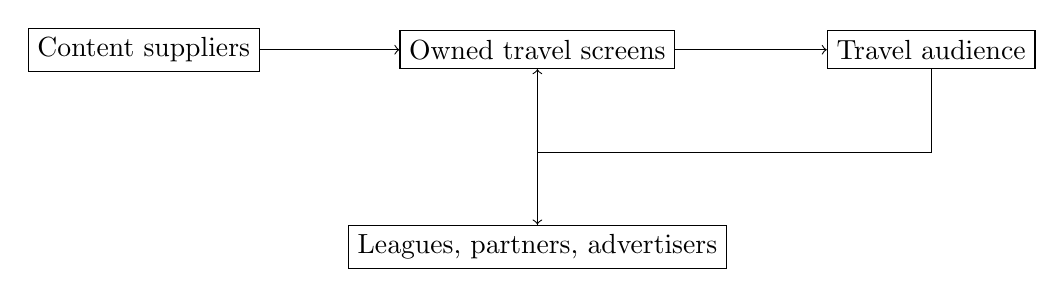
\begin{tikzpicture}
\node[draw, rectangle] (content) at (0,0) {Content suppliers};
\node[draw, rectangle] (network) at (5,0) {Owned travel screens};
\node[draw, rectangle] (aud) at (10,0) {Travel audience};
\node[draw, rectangle] (adv) at (5,-2.5) {Leagues, partners, advertisers};
\draw[->] (content) -- (network);
\draw[->] (network) -- (aud);
\draw[->] (aud) -- +(0,-1.3) -| (adv);
\draw[->] (adv) -- (network);
\end{tikzpicture}
\end{figure}

\subsection{Question \& Answer}

\paragraph{Question.} How do we win in a crowded market without merely outspending the incumbents?

\paragraph{Answer.} The lecture's answer is to control the interface through which everybody else must pass. Once that interface is controlled, competitors may become customers, partners may become distributors, and attention itself becomes an asset.

This is where the lecture recovers, at a higher level, the same deep structure we saw in dry cleaning. There the factory turned competitors into wholesale customers. Here the travel screens turn leagues, partners, and other market participants into intertwined counterparties. Control the scarce middle, and the boundary between rival and customer becomes porous.

The founder's advice on selling and negotiating fits the same pattern. Serve the person in front of you. Never do something to somebody; do something for someone. And when a prospective client leans toward no, the same old rule returns: no is not the end state; it is not yet. Thus the lecture's persistence principle, first learned in the street hunt, reappears as a principle of commercial negotiation.

The network motif also becomes explicit here. The founder says he has kept the same phone number for decades and can call anyone; your net worth is really your network. The line can sound like a cliche until he explains the operational core of it: show up where you are supposed to be, again and again, in person, until other people recognize your commitment before they commit to you. Network depth is not social sparkle. It is accumulated availability.

\section{Private Equity, Actual Cash Flow, and the Final Finance Lens}

The final interview is analytically distinct. The guest is in private equity, not yet at a first million, and for that very reason the lecture closes with a cleaner financial vocabulary rather than with another maximal success story. Asked what he would do if he were starting over, he answers: boring businesses that make real cash flow, and financial-services businesses that can achieve scale. Real assets, data centers, waste management, and similar activities are preferable to stories that sound impressive but do not underwrite well.

\subsection{Question \& Answer}

\paragraph{Question.} If we were starting over, what exactly should we optimize for: glamour, growth stories, or cash that can actually be underwritten?

\paragraph{Answer.} The lecture's answer is unromantic and therefore useful. It prefers actual cash generation to EBITDA-style appearance. The latter is described in the interview as ``kind of fake cash flow.'' The safe mathematical version is not that EBITDA is meaningless, but that debt capacity depends more directly on actual cash generation:
\begin{align}
CF_{\text{actual}} &\not\equiv E_{\text{EBITDA}}, \\
D_{\max} &= f(CF_{\text{actual}}), \qquad f' > 0.
\end{align}
That is, leverage follows serviceable cash, not the most flattering accounting story.

The bank example sharpens the point. Banks lend to make money, and they do so on the spread:
\begin{equation}
s_{\text{bank}} = r_{\text{loan}} - r_{\text{funding}}.
\end{equation}
The lecture does not write this as a textbook formula, but that is what its intuition amounts to. The mystique is stripped away: the institution earns the margin between what it charges and what it pays.

\begin{remark}
The lecture's dismissal of EBITDA should be read heuristically. The narrower and safer claim is that lenders and acquirers ultimately care about cash that can service obligations.
\end{remark}

Several other themes now tighten. Networking got this guest into private equity. Team quality is how one stands out in a competitive market. Finding deals and matching those deals with money is the scaling task. The most memorable metaphor is that one should think about money the way one thinks about air. This is not an equation and should not be over-literalized. It means only that the desired state is one in which money ceases to be a constant obsession because the system generating it is already working.

It is also fitting that the lecture ends with a guest who has not yet crossed the first-million threshold. The point is not that the lecture wants less success at the end. The point is that the final guest offers a language in which the earlier interviews can be restated: boring cash flow, debt capacity, spread, team, network, and the difference between real dollars and flattering narratives.

\section{Summary}

The lecture begins with a street question and ends with a financial grammar, but it never loses the order in which its ideas are earned. First we learn that access itself is scarce and persistence is part of the method. Then, through the dry-cleaning case, we see that scale often means separating the indispensable core from the many lightweight edges. After that the lecture asks the more difficult question: how does a first million become a durable flow? The answer, at least initially, is behavioral rather than portfolio-theoretic. The surgeon then gives us a second model, in which professional expertise becomes entrepreneurial wealth through purpose, quality, trust, and the leap of starting one's own practice. The Reach TV founder lifts the whole picture to distribution, rights windows, and network power. Finally the private-equity guest strips the glamour away and asks us to underwrite actual cash.

\begin{table}[h]
\centering
\begin{tabular}{llll}
\hline
Case & First million & Business & Mechanism \\
\hline
Dry-cleaning owner & about 10 years ago & Dry cleaning, later tech & Own the factory; scale the intake nodes \\
Spine surgeon & effectively last year & Medical practice & Start the practice; let service quality sell \\
Reach TV founder & about age 28 & Travel television network & Control the rights window and audience \\
Private-equity operator & not yet & Real-assets private equity & Prefer actual cash flow to accounting gloss \\
\hline
\end{tabular}
\end{table}

If we want one compact sentence to carry the chapter, it is this: durable wealth comes from repeatable systems. Those systems may take the form of a factory, a medical practice, a controlled distribution channel, or a portfolio of boring cash-flow businesses, but in every case the lecture pushes us away from spectacle and toward mechanism.